\section{Introduction}
\label{sec:intro}

Object recognition, object detection, object tracking, object discovery, action recognition and other high-level visual tasks can benefit from an intermediate level representation that potentially represents objects or object parts. The act of identifying regions in the image that potentially correspond to objects is known as generating \emph{object proposals}~\cite{Malisiewicz:Efros:BMVC07, Alexe:etal:PAMI12, Endres:Hoiem:PAMI14, Carreira:Sminchisescu:PAMI12, Chang:etal:ICCV11, Rahtu:etal:ICCV11,Zhang:Torr:PAMI16, Feng:etal:ICCV11, Uijlings:etal:IJCV13, Narayanan:Kimia:ECCV12, Kim:Grauman:ECCV12, Manen:etal:ICCV13, Humayun:etal:CVPR14, Arbelaez:etal:CVPR14, Rantalankila:etal:CVPR14, Krahenbuhl:Koltun:ECCV14, Bonev:Yuille:ECCV14, Zitnick:Dollar:ECCV14, Cheng:etal:CVPR14, Erhan:etal:CVPR14, Krahenbuhl:Koltun:CVPR15, Xiao:Lu:etal:CVPR15, Chen:etal:CVPR15, Lu:etal:ICCV15, Humayun:etal:ICCV15, He:Lau:ICCV15}. While the current paradigm of decomposing an image into a set of \emph{object proposals} is popular among many different computer vision tasks the evolution to this now accepted intermediate from originates from the difficulties faced with ``sliding-window'' approaches in object detection.

Until most recently, the most successful approaches to object detection have all utilized the well known, ``sliding window'' paradigm~\cite{Papageorgiou:Poggio:IJCV00,Viola:Jones:IJCV04,Felzenszwalb:PAMI:09} in which a learned classifier tests for the presence of an object in every sampled candidate image window. In a general object detection setting, the number of candidate windows tested must be performed over all possible object positions, scales, and aspect ratios. The linear complexity of ``sliding window'' approaches with respect to the size of this 4-dimensional search space,$(x,y,w,h)$, makes it difficult to efficiently search over all possible windows. Even if the number of candidate windows was minimal the exponential growth in dataset sizes has naturally forced classifiers to become more sophisticated at the expense of increased computational run-time to evaluate a single window. Given that it is intractable to exhaustively evaluate these more complex classifiers over millions or possibly billions of image windows researchers have developed heuristics to speed up the search, at the risk of possibly mislocating or missing objects altogether. While there have been more structured approaches such as Branch and Bound~\cite{Lampert:etal:PAMI09} that do no resort to these heuristics, all ``sliding window'' approaches are forced to make trade-off's between  detection quality and computational tractability.  Overcoming this trade-off was the major driving factor toward the research and development of \emph{object proposals}. 

\emph{Object proposal} methods overcome this trade-off by utilizing segmentation as a pre-processing step to generate a small of pool candidate regions (on the order of thousands) that are then passed into various classification algorithms. Reasoning with this reduced set of regions allows ``sliding window'' approaches to bypass the need for searching over the space of all candidate windows. While the idea of utilizing segmentation as a precursor to recognition is not a novel idea the difficulties faced with classic segmentation rendered this paradigm moot. Two major leaps in thinking essentially overcame the difficulties in traditional segmentation and are the basis for all \emph{object proposal} schemes. The first major leap in thinking was the Soup of Segments~\cite{Malisiewicz:Efros:BMVC07} work which argued that rather than generate a single segmentation we should generate a diversity of segmentations. By exploring multiple segmentations we increase the likelihood of finding objects that are perfectly segmented in one partitioning but erroneously merged or broken in other segmentations. The second major idea was first made in 2010 concurrently by three independent groups, {\bf Objectness}~\cite{Alexe:etal:PAMI12}, {\bf CPMC}~\cite{Carreira:Sminchisescu:PAMI12}, and {\bf Category Independent Proposals}~\cite{Endres:Hoiem:PAMI14}. The key observation was that if our goal in subsequent processing is object centric tasks (recognition, detection, \etc) why focus on exhaustively partitioning, , Figure~\ref{fig:diffs}\textcolor{red}{(a)}, every pixel into a unique region? Rather we should focus on directly generating a pool of \emph{proposals} (bounding box or free-form regions), Figure~\ref{fig:diffs}\textcolor{red}{(c,d)}, that are likely to capture \emph{objects} in the scene without providing a complete image segmentation. By relaxing the original segmentation formulation to only focus on object-like area's of the image coupled with exploring multiple possibly overlapping segments the problem becomes more forgiving and we have a much greater chance of generating good proposals. 

\begin{figure}[ht]
\centering
{\footnotesize\textit{a)}}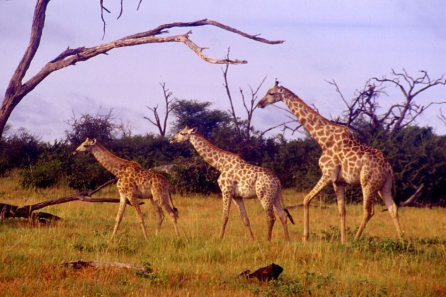
\includegraphics[width=0.228\textwidth]{figs/three.jpg}
{\footnotesize\textit{b)}}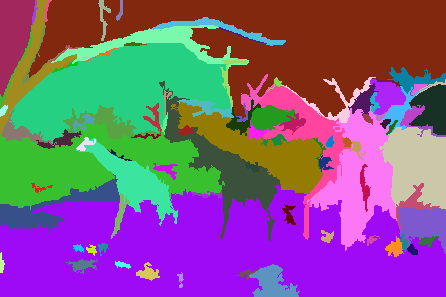
\includegraphics[width=0.228\textwidth]{figs/out.png}
{\footnotesize\textit{c)}}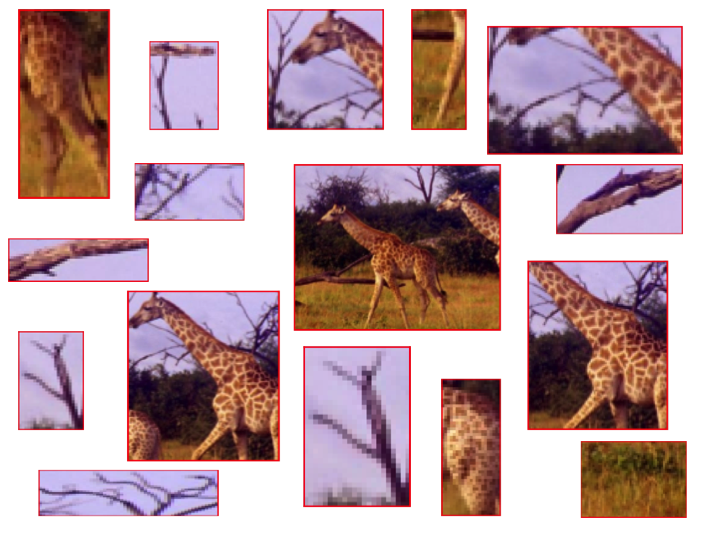
\includegraphics[width=0.228\textwidth]{figs/giraffe_bbox.png}
{\footnotesize\textit{d)}}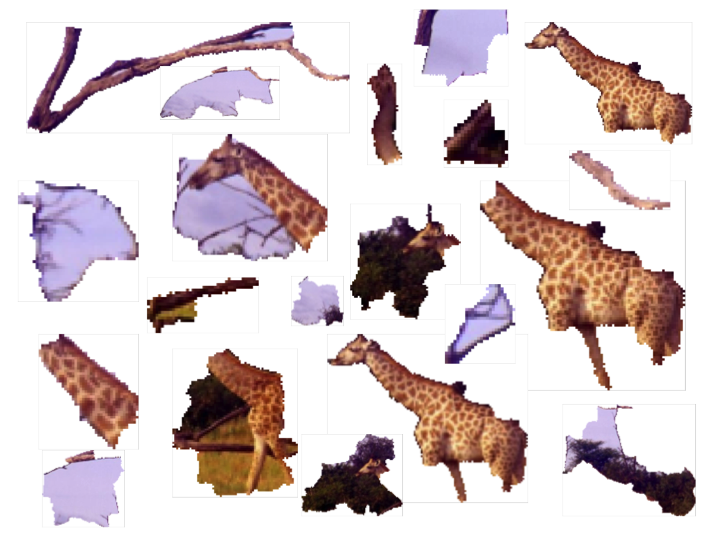
\includegraphics[width=0.228\textwidth]{figs/giraffe_ops.png}
\caption{a) Image and classical segmentation in b). We see the object proposal representation in c) and d).}
\label{fig:diffs}
\end{figure}

\begin{figure}[ht]
\centering
{\footnotesize\textit{a)}}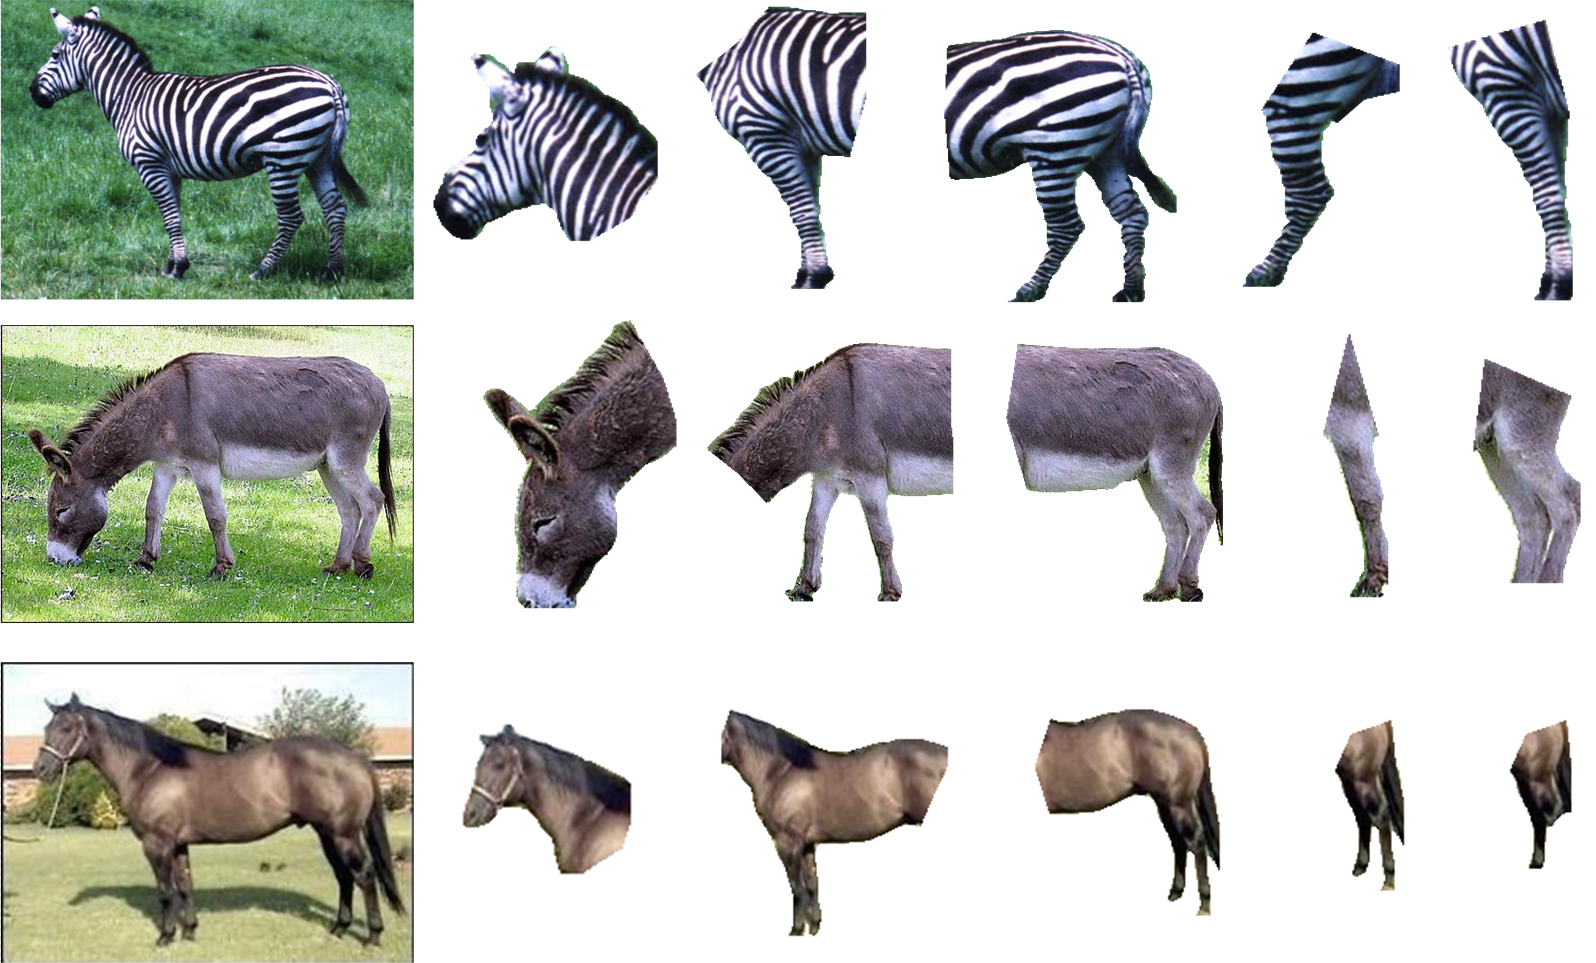
\includegraphics[width=0.229\textwidth]{figs/all_frags_per_image_part1.png}
{\footnotesize\textit{b)}}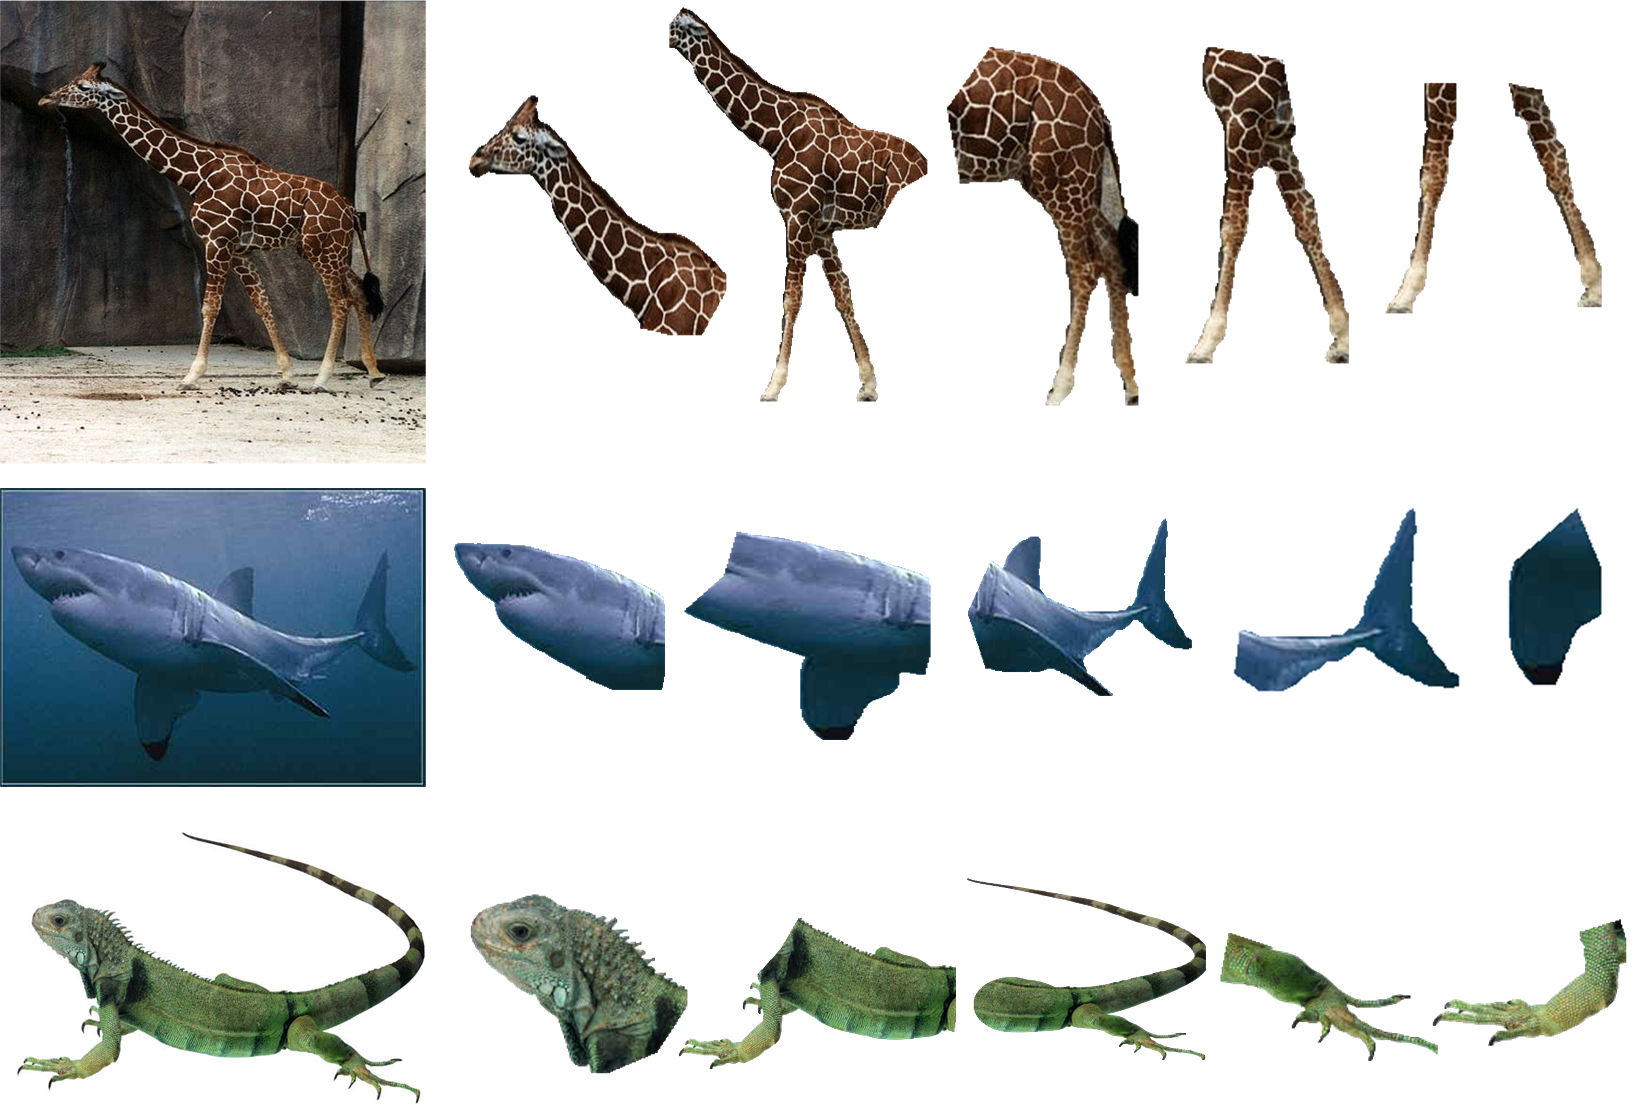
\includegraphics[width=0.229\textwidth]{figs/all_frags_per_image_part2.png}
{\footnotesize\textit{c)}}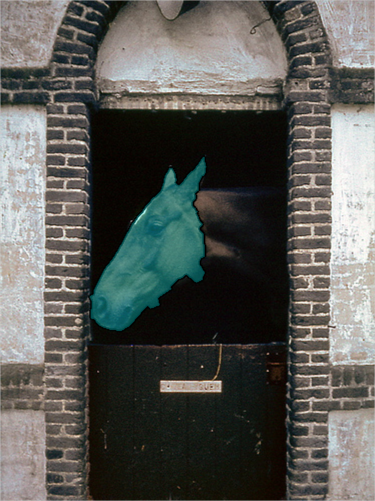
\includegraphics[height=0.13\textheight]{figs/horse_occlude.png}
{\footnotesize\textit{d)}}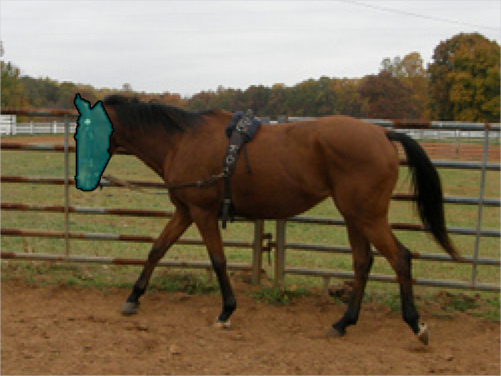
\includegraphics[width=0.235\textwidth]{figs/horse_no_occlude.png}
\caption{Examples of various part based object proposals generated by our approach in (a) and (b). For clarity, proposals from the background and full-object proposals are not shown. In (c) only a portion of the horse is shown due to occlusion while in (d) the full horse is recoverable. To correlate the two we must be able to recover the portion, head, of the objects visible in both images. The head is in highlighted in cyan. }
\label{fig:part_ops}
\end{figure}

Our work is distinct in both its goal and approach. The primary application of object proposals has been in object detection. As such, approaches have focused on recovering full object proposals in a scene, \ie, the three giraffes in Figure~\ref{fig:diffs}\textcolor{red}{(a)}. Our primary goal, however, is to recover parts and their combinations, \ie, legs, heads, tails, legs plus body, head plus neck, \etc, Figure~\ref{fig:part_ops}\textcolor{red}{(a,b)}. Part-based object proposals have received considerable less attention in the object proposal literature. Our motivation for focusing on parts is that the problem is much more tractable than trying to recover full objects. Furthermore, the recovery of parts is important when trying to correlate object proposal across scenes with varying degrees of occlusion, Figure~\ref{fig:part_ops}\textcolor{red}{(c,d)}. 



%% {\bf One of the major contributions of our work is to show how our approach is flexible enough to recover part-based proposals along with full object proposals.} 


\begin{figure}[ht]
\centering
{\footnotesize\textit{a)}}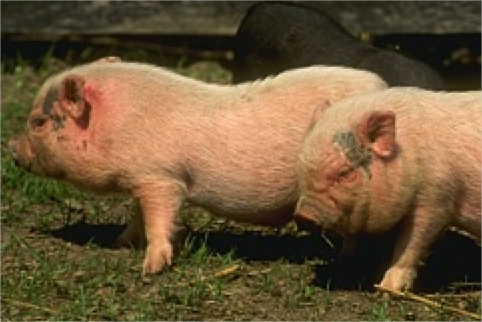
\includegraphics[width=0.229\textwidth]{figs/piggies.png}
{\footnotesize\textit{b)}}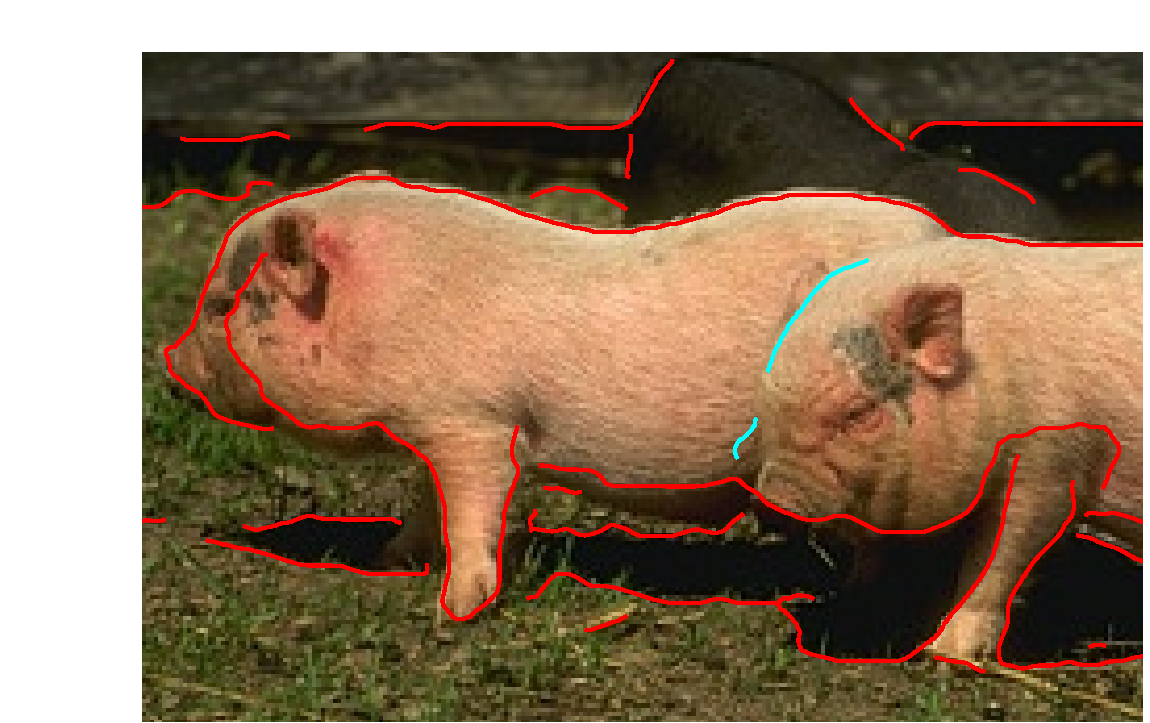
\includegraphics[width=0.229\textwidth]{figs/piggies_cons.pdf}
{\footnotesize\textit{c)}}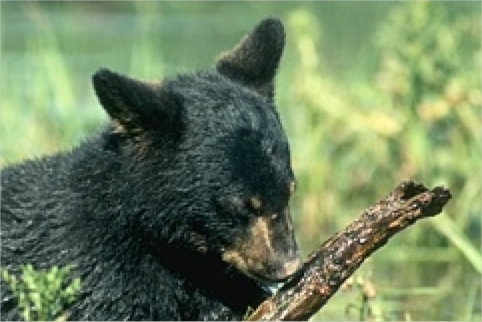
\includegraphics[width=0.229\textwidth]{figs/bear_head.png}
{\footnotesize\textit{d)}}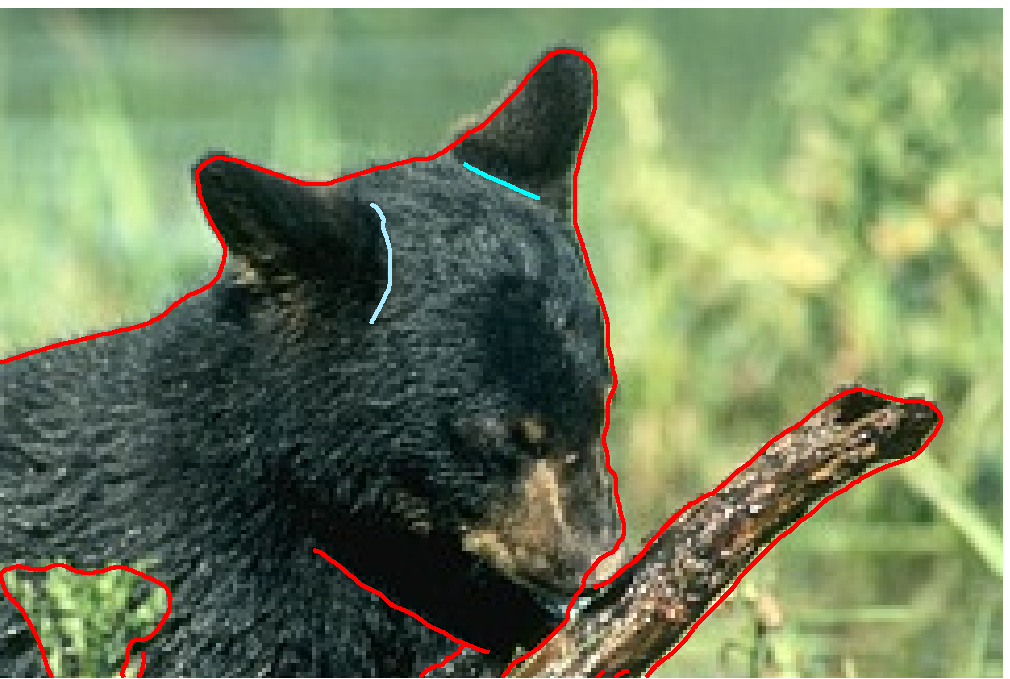
\includegraphics[width=0.229\textwidth]{figs/bear_head_cons.pdf}
{\footnotesize\textit{e)}}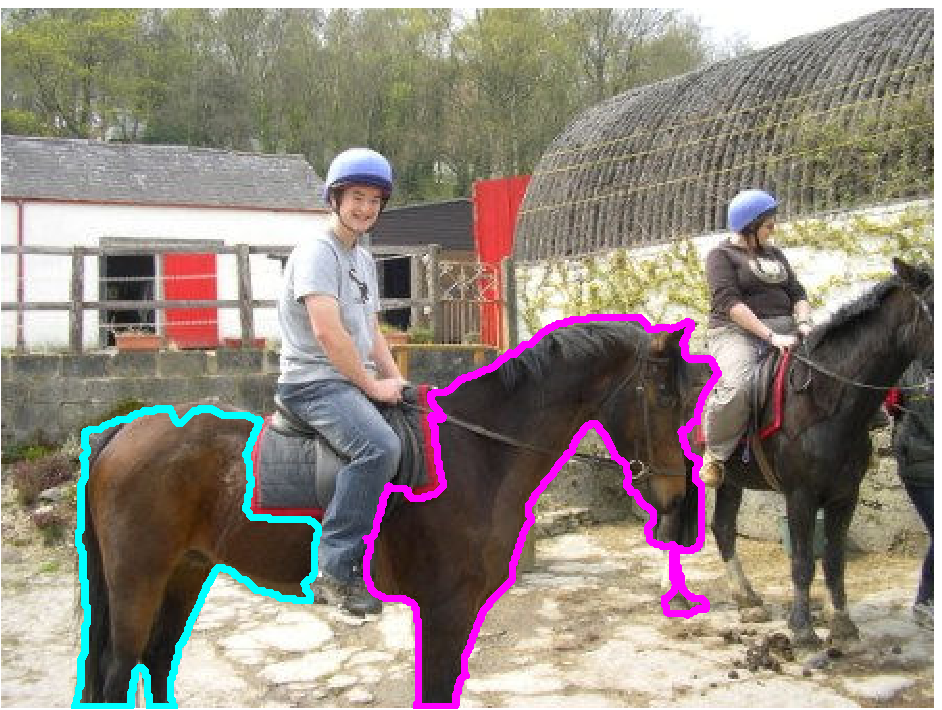
\includegraphics[width=0.229\textwidth]{figs/horse_occluded.pdf}
\caption{Reasoning with a purely regional representation of (a) will lead to the two pigs being merged as the two pigs are roughly homogenous. (b) If we consider a contour representation of the objects we see that the presence of the internal \textcolor{cyan}{cyan} provides a clue to the delineation of the two pigs. In (c) we see how a purely regional representation could lead to the ears merging with the rest of the bear head, but the \textcolor{cyan}{contours} in (d) roughly fall along the part lines of the ear. (e) We observe how purely reasoning with contour cues does not merge the two horse parts} 
\label{fig:cons_vs_regions}
\end{figure}

The majority of object proposal approaches are based on revisiting region-based segmentation in the context of recovering object proposals. As such approaches have repurposed the same regional representations of an image, Region-Adjacency Graph (RAG) of pixels or superpixels, region hierarchies, \etc, for the recovery of object proposals. An implicit assumption of these representations is that objects in a scene are exclusively defined by their regional signature, cohesive areas of color and texture, and the recovery of object proposals is simply a manipulation of this underlying representation, \ie, merging pixels or superpixels, partitioning the graph using graph cuts, \etc. This ignores the contour signature, silhouette curves, objects leave behind in their projection onto an image. Observe that in Figure~\ref{fig:cons_vs_regions}\textcolor{red}{(a)} a purely regional representation of the image could lead to the two pigs being merged as the objects are roughly homogenous in appearance. If we consider the contour signature, Figure~\ref{fig:cons_vs_regions}\textcolor{red}{(b)}, observe that the silhouette of the pig head is recovered, highlighted in \textcolor{cyan}{cyan}, providing strong evidence for the separation of these regions. The role of contours is even more important in the recovery of parts. Figure~\ref{fig:cons_vs_regions}\textcolor{red}{(c)} shows a black bear of roughly uniform appearance. While a regional representation could lead to the ears, head, and body merging the contour signature, Figure~\ref{fig:cons_vs_regions}\textcolor{red}{(d)} identifies internal contours, highlighted in \textcolor{cyan}{cyan}, falling along the part lines separating the head from the ear. While contour signatures are important regional signatures are still key. Observe in Figure~\ref{fig:cons_vs_regions}\textcolor{red}{(e)} the recovery of the full horse is occluded by the rider. While a contour representation can recover the two pieces, highlighted in cyan and magenta, the main cue to unify these two parts is the regional homogeneity. Finally, a more recent trend as proposed by~\cite{Bonev:Yuille:ECCV14} is to also recover contextual or background fragments, sky, grass, \etc. The recovery of these background proposals which lack any clear defined silhouette are better recovered by exclusively reasoning with the regional attributes. This is not just the old tale of integrating contours and regions, but rather the simultaneous representation of both. To do that we propose a new multi-faceted representation that captures both signatures in a unified fashion. 

%% {\bf One of the major contributions of our work is to propose a new multi-faceted representation that overcomes the limitations of current region and contour based representations.}

 
The second distinction between our approach and others is how we reason with our representation to generate object proposals. One of the key requirements of object proposals schemes is to achieve high recall, \ie, ALL objects in a scene should be recovered with sufficient quality. To satisfy this requirement a large pool of candidate proposals is generated with the assumption that if the pool is sufficiently large all objects in the scene will be recovered with high probability. Building off the Soup of Segments approach~\cite{Malisiewicz:Efros:BMVC07} this pool is generated by sweeping the parameters that govern that particular algorithm. In this view, each object proposal is generated by some combination of algorithm settings and the sweep of all possible parameters settings generates a set of possible object proposals. The difficulty of this approach is that there is no guarantee that objects will exactly map to some combination of parameters, and across datasets it is not clear how generalizable the parameter settings will be. 

\begin{figure*}[ht]
\centering
{\footnotesize\textit{a)}}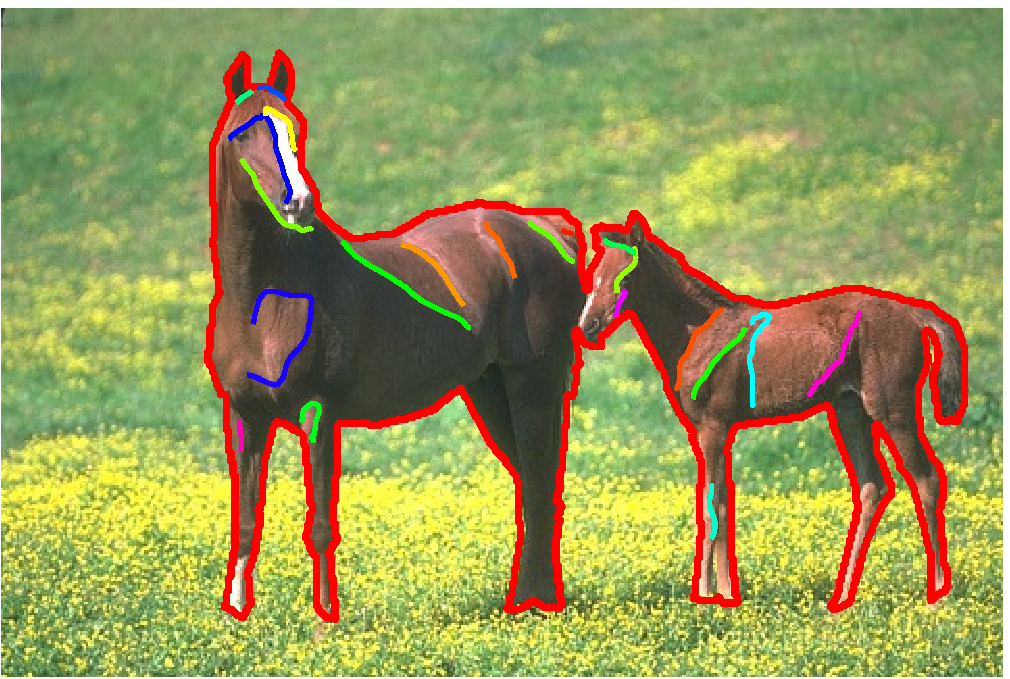
\includegraphics[width=0.241\textwidth]{figs/ic_horses.pdf}
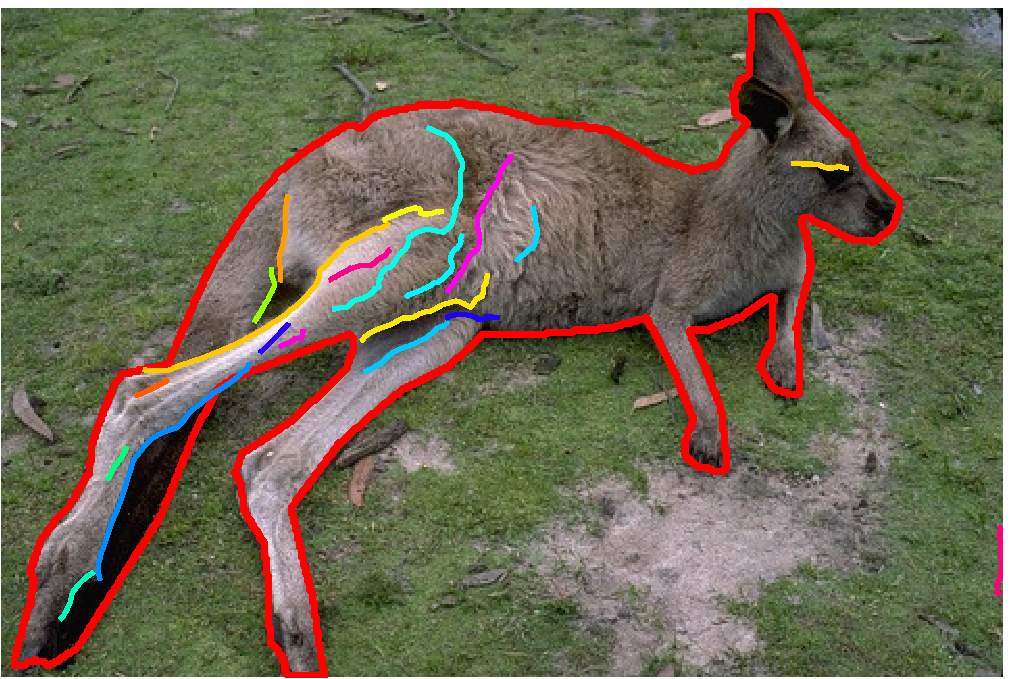
\includegraphics[width=0.241\textwidth]{figs/ic_kang.pdf}
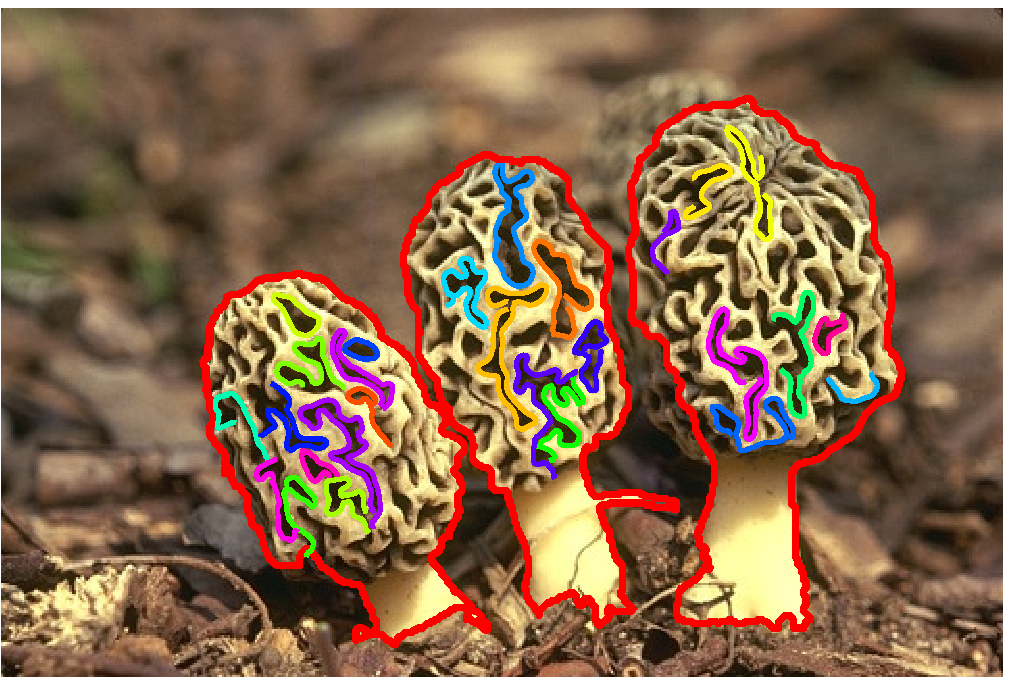
\includegraphics[width=0.241\textwidth]{figs/ic_mush.pdf}
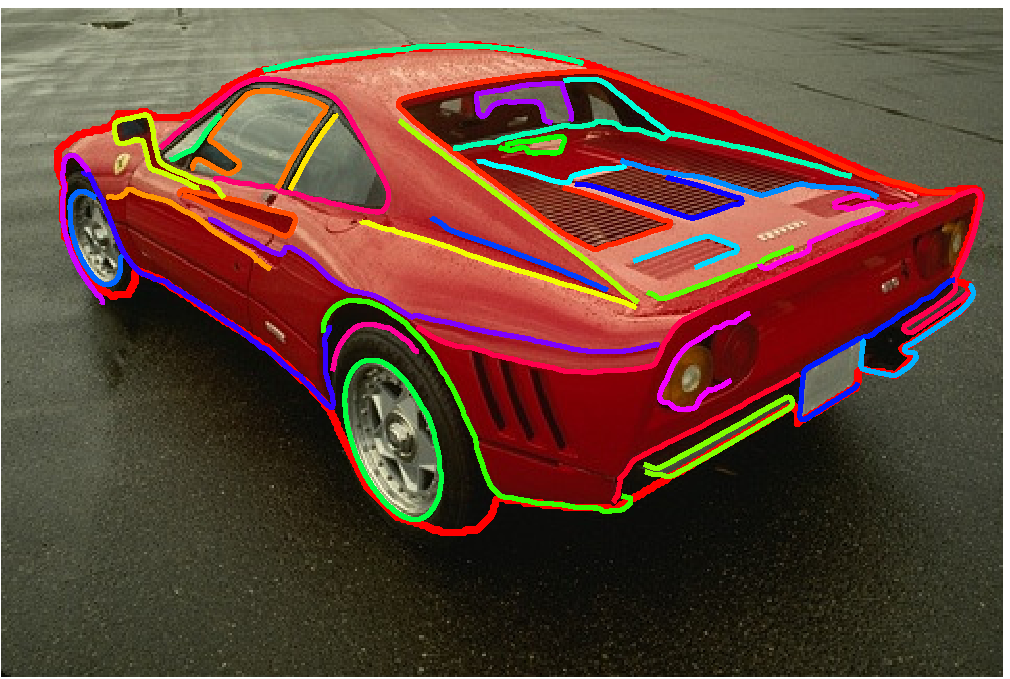
\includegraphics[width=0.241\textwidth]{figs/ic_car.pdf}
{\footnotesize\textit{b)}}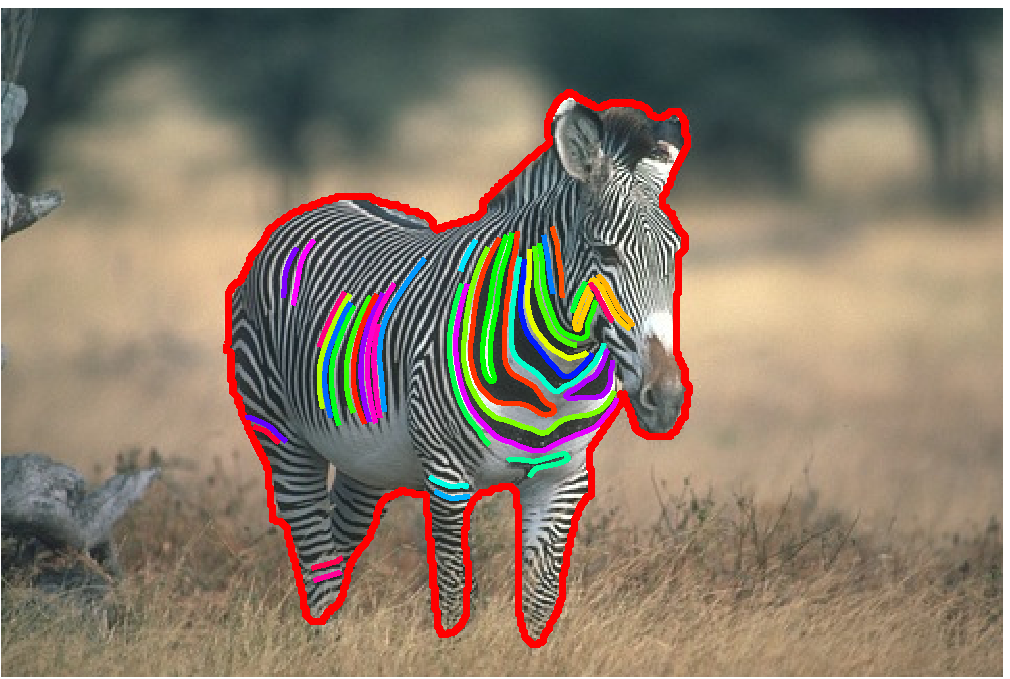
\includegraphics[width=0.241\textwidth]{figs/rr_stripes.pdf}
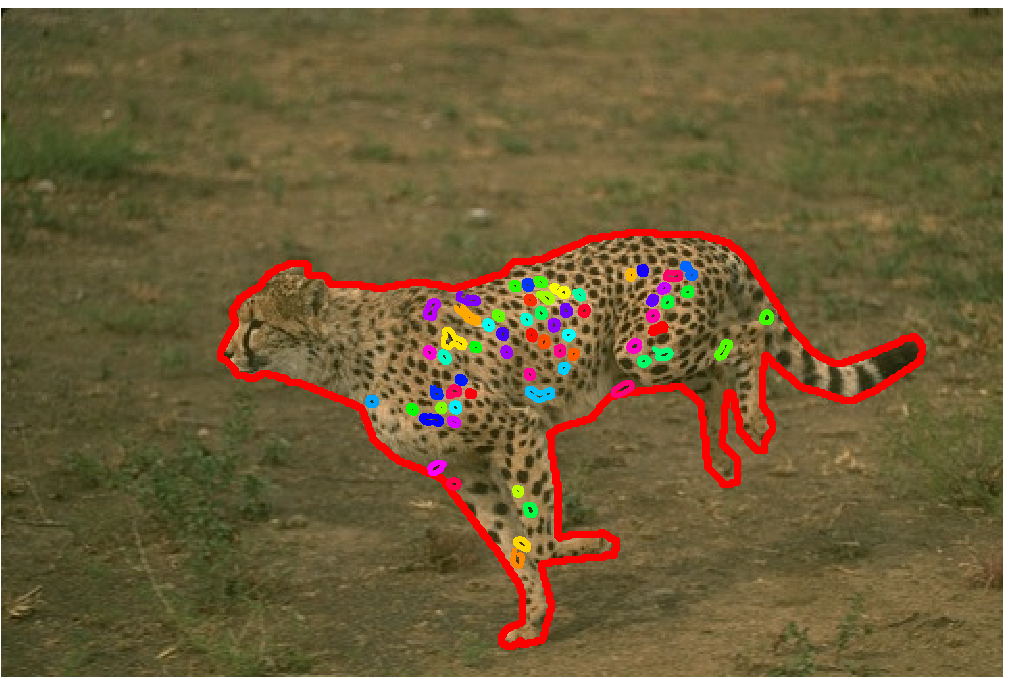
\includegraphics[width=0.241\textwidth]{figs/rr_spots.pdf}
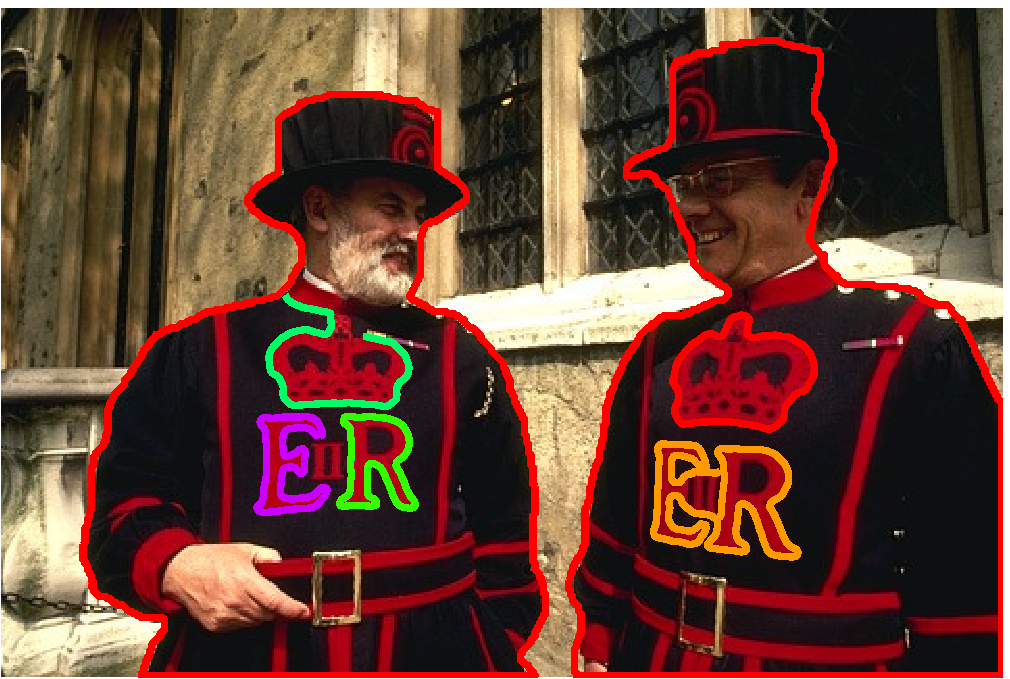
\includegraphics[width=0.241\textwidth]{figs/rr_markings.pdf}
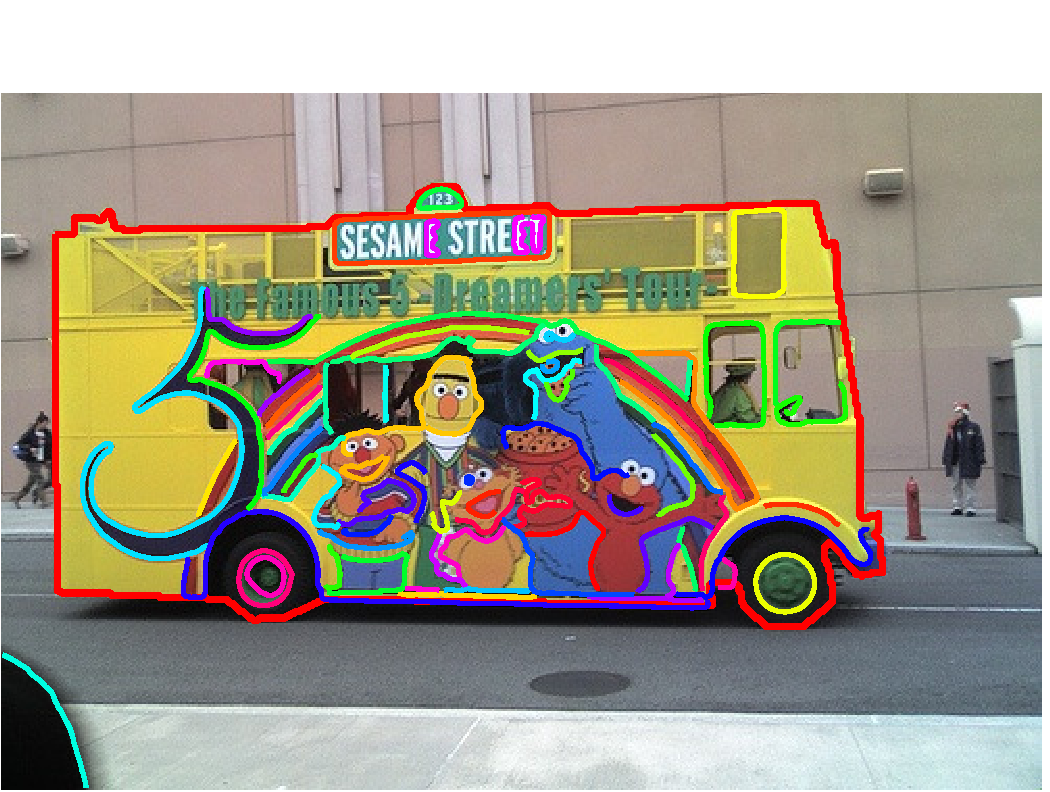
\includegraphics[width=0.241\textwidth]{figs/rr_bus2.pdf}
{\footnotesize\textit{c)}}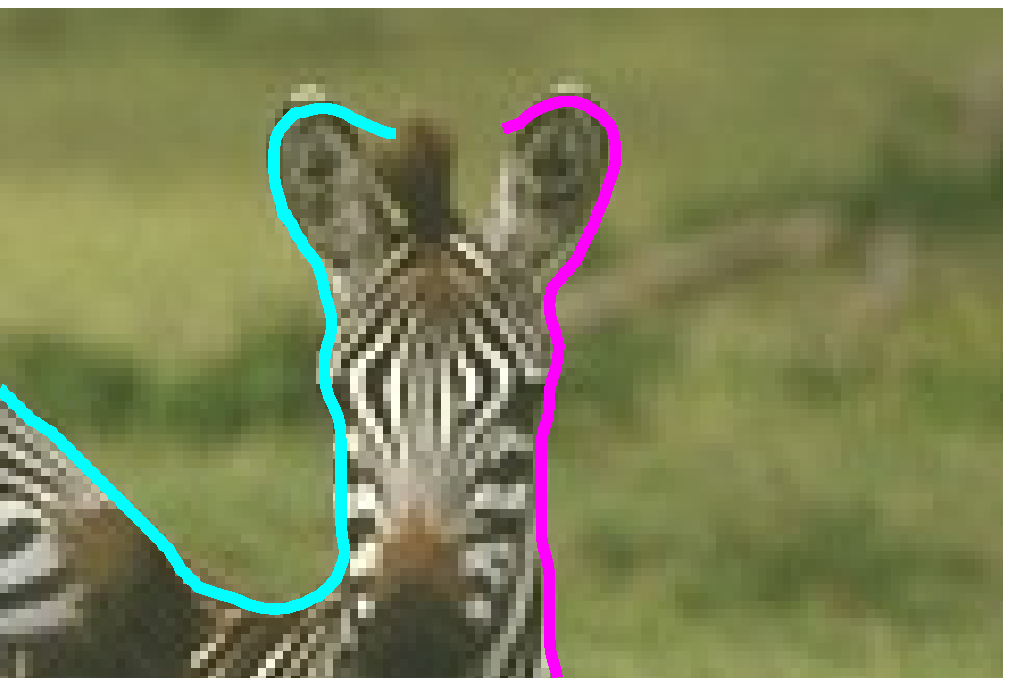
\includegraphics[width=0.241\textwidth]{figs/zebra_miss.pdf}
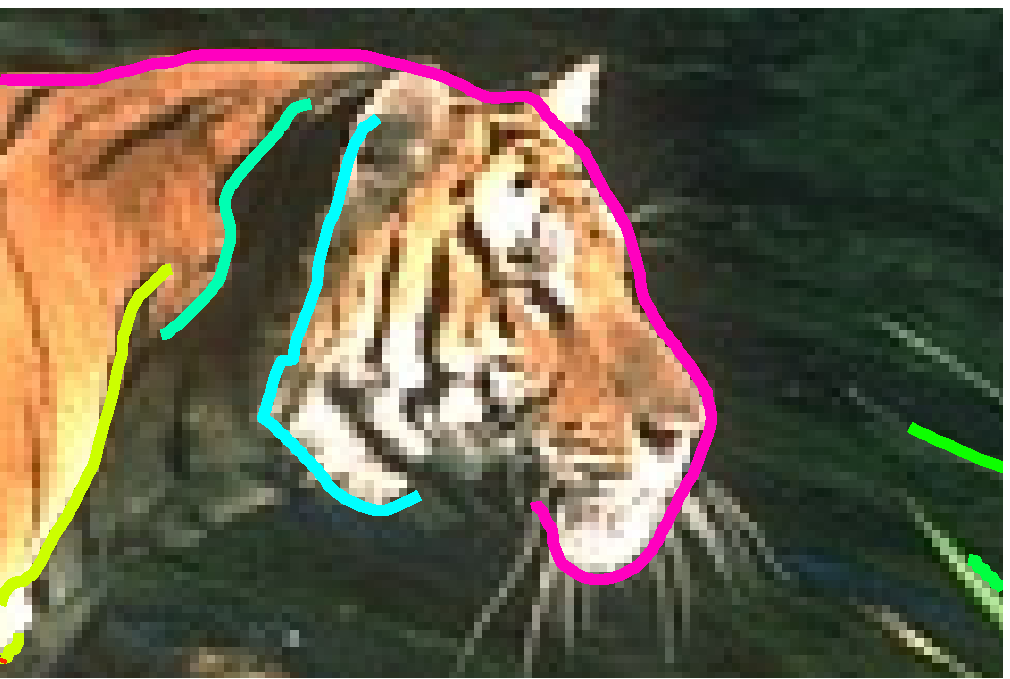
\includegraphics[width=0.241\textwidth]{figs/tiger_miss.pdf}
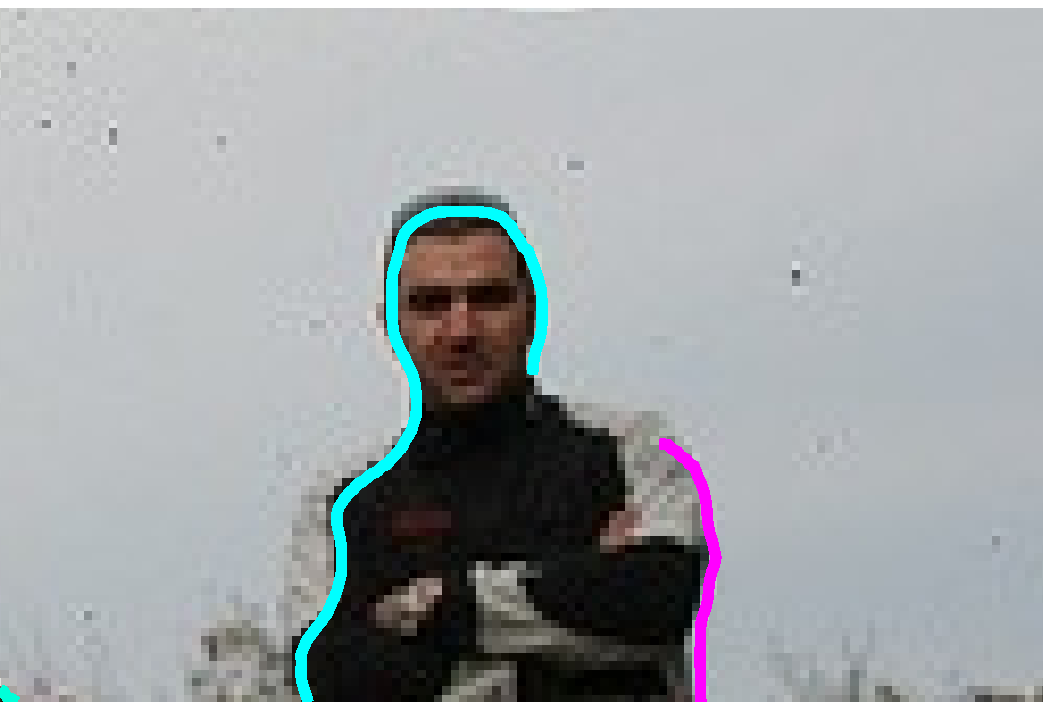
\includegraphics[width=0.241\textwidth]{figs/person_miss.pdf}
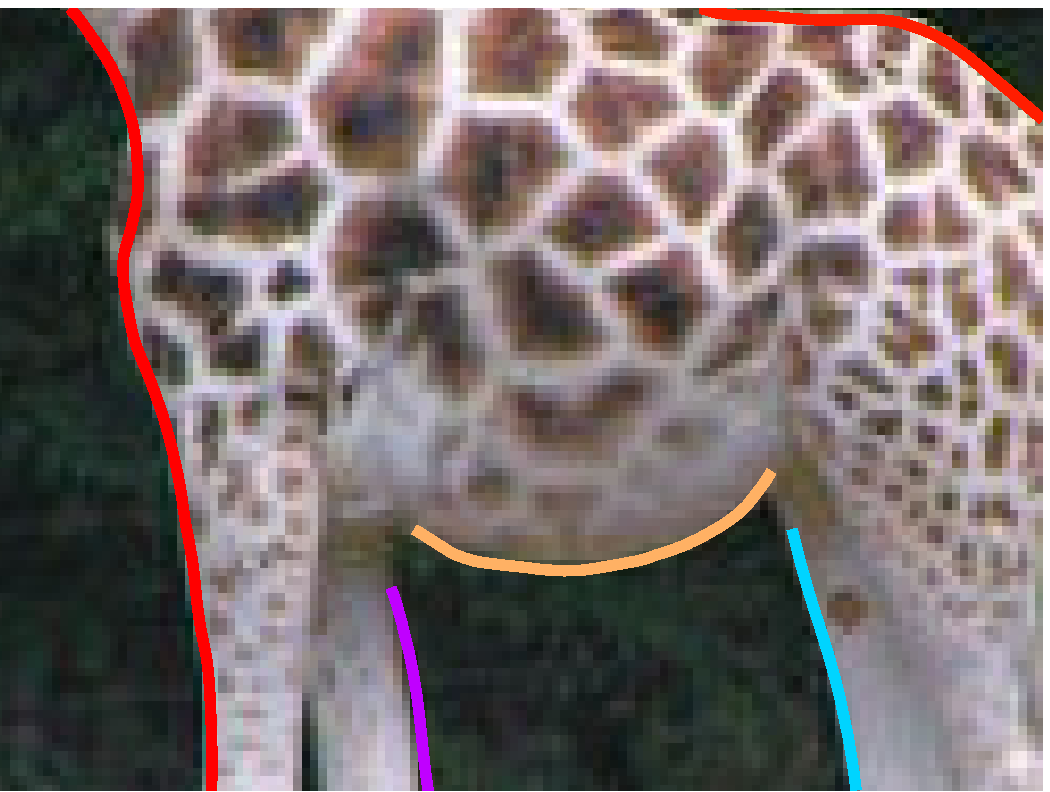
\includegraphics[height=0.16\textwidth]{figs/giraffe_miss.pdf}
{\footnotesize\textit{d)}}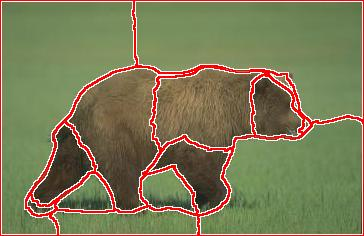
\includegraphics[width=0.243\textwidth]{figs/bear_segment.jpeg}
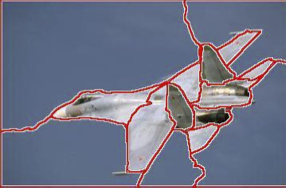
\includegraphics[width=0.243\textwidth]{figs/plane_segment.png}
\caption{We observe various examples of degradations to ideal signatures of objects in a scene. a) Despite ideal silhouettes, highlighted in red, \emph{clutter contours}, randomly colored, interrupt the recovery of the full object. b) Observe that \emph{clutter regions} interrupt the recovery of objects despite ideal silhouettes. c) The ideal silhouette is interrupted by \emph{contour gaps}. d) We see roughly homogenous objects disjointed into various regions that need to be merged to recover the whole. These results were illustrated with N-Cuts~\cite{Shi:Malik:PAMI00}, but the principle is the same irrespective of segmentation algorithm. } 
\label{fig:trans_examples}
\end{figure*}

In our work, we deviate drastically from this canonical view, and take a more structured approach where we look at the formation of object and part proposals as the process of recovering the ideal signatures (contour and region) given an image where object signatures have been degraded. Consider Figure~\ref{fig:trans_examples} where we see how the dual signatures of objects in a scene are distorted due to various imaging and scene affects. In Figure~\ref{fig:trans_examples}\textcolor{red}{(a,b)} we see how despite recovering an ideal contour silhouette, highlighted in red, the recovery of the full object and its parts is interrupted by the presence of \emph{contour-clutter} and \emph{region-clutter} respectively. For example, the muscles of the horse in Figure~\ref{fig:trans_examples}\textcolor{red}{(a)} lead to the formation of internal contours while the recovery of the people and bus in Figure~\ref{fig:trans_examples}\textcolor{red}{(b)} is interrupted by regional surface markings. In Figure~\ref{fig:trans_examples}\textcolor{red}{(c)} we we observe that even if we don't have any \emph{contour-clutter} or \emph{region-clutter} the ideal silhouette can be interrupted causing \emph{contour gaps} to form. Observe that the silhouettes of the zebra head, tiger head, and person are interrupted. And finally an ideal picture of a large homogenous region is unnecessarily disjointed due to scene and imaging effects disrupting the underlying appearance characteristics, Figure~\ref{fig:trans_examples}\textcolor{red}{(d)}. To recover the objects and parts in a scene we adopt a \emph{perceptual organization} approach where each of the degradations illustrated in Figure~\ref{fig:trans_examples} are dealt with in a Gestalt framework. For example, to recover the horse or person we must remove the clutter contours and clutter regions respectively, or we must complete gaps in the case of Figure~\ref{fig:trans_examples}\textcolor{red}{(d)} to recover the zebra head, tiger head, and human outline or finally some combination of these counter-actions is needed to recover more complex objects in a scene. This quickly leads to a large number of possibilities. These various grouping options are efficiently tracked and the entire set of options are maintained. This is an important distinction because while it is possible that viable fragments are not formed under the variations-of-variables scheme (\eg, object was too small and no seeds were initialized inside), it is much less likely that viable fragment would avoid being considered due to the structural and exhaustive nature of the proposed scheme. 

In summary, our main contributions are:

\begin{itemize}

\item A new multi-faceted representation that overcomes the limitations of current region and contour based representations (Section~\ref{sec:atomic:fragments}). 

\item The formalization of a new perceptual organization framework that maps high-level image degradations (presence of clutter, interruptions in contours, \etc) to a concrete set of contour-actions (transforms) (Section~\ref{sec:transforms}). 

\item An efficient strategy to practically explore the expansive and conflicting set of grouping options our Gestalt framework puts forth (Section~\ref{sec:cgraph}). 



\end{itemize} 
%% {\bf One of the major contributions of our work is to formulate a perceptual organization framework that maps each degradation (clutter, gaps, etc) to a corrective action.} 


%% The horse, zebra, mushroom, and car are interrupted with various “clutter” contours while various regions inhibiting the recovery of full objects interrupt the objects in the second row. The third and fourth row sow how object signatures can be interrupted by gaps, and finally similar to region based schemes we need to merge regions. To deal with all these degradation's of objects in a scene we exploit certain regularities as advocated by Gestalt psychologists  

%% There are a varied set of approaches to generate object proposals. Despite different formulations all object proposals follow the same basic framework. Methods generate a diverse set of multiple candidate regions or bounding boxes by varying the specific parameters that govern the particular proposal generation algorithms. In this view, each object proposal is generated by some combination of algorithm settings and the sweep of all possible parameters settings generates the space of all possible object proposals. The final output proposals can then be seen as a sampling of this space. In our work, we deviate drastically from this canonical view, and look at each object proposal and the generation of multiple object proposals as the result of \emph{perceptual organization} of the image. 

%% \textcolor{red}{To Ben: This next paragraph is from our ECCV'12 intro}
%% \\
%% \indent
%% Our approach is distinct in several ways:\   First,
%% previous work aims to generate full object hypotheses, while we aim to generate
%% recognizable and meaningful object part hypotheses. Second, previous work
%% generates multiple hypotheses by varying segmentation variables such as parameters, algorithms, seeding, {\emph{etc.,}} while we systematically and exhaustively investigate all reasonable
%% grouping options in a 
%% perceptual reasoning Gestalt framework, by asking questions like: what if these contour fragments are bridged across a gap? What if this contour fragment is spurious? These possibilities are all methodically tracked and the entire sets of options are maintained! This is an important distinction because while it is possible that viable fragments are not formed under the variations-of-variables scheme (e.g., object was too small and no seeds were initialized inside), it is much less likely that viable fragment would avoid being considered due to the structural and exhaustive nature of the proposed scheme.  

%% Our major contribution is to take a more structured approach to the formation of objects proposals. 


%% The implicit assumption in all existing schemes is that objects of interest exist



%%  To generate a single object, whether segment or bounding box, 

%% that object proposals take to generate object proposal 
 
%% While object proposals scheme differ on the appropriate proposal representation, segment or bounding box, all objects proposals are consistent in how they generate a \emph{diverse} set of proposals. In the “Soup of Segments” approach a \emph{diverse} set of segments is generated by inducing variations in the segmentation procedure by using complementary segmentation algorithms, changing the segmentation parameters or seeding, and by merging adjacent segmented regions. Building on the work of Soup of Segments, object proposal schemes generate a diverse set of multiple candidate regions by varying the specific parameters that govern the particular proposal generation algorithms. In this view, each object proposal is parameterized by some combination of algorithm settings and the sweep of all possible parameters settings generates the space of all possible object proposals with the output proposals being a sampling of this space. In our work, we deviate drastically from this canonical view, and 

%% This canonical view of all object proposals 


%% For example, one of the most popular approaches, SelectiveSearch, 

%% Given an image, all object proposal schemes, attempt to generate a small diverse set of possibly overlapping proposals that hopefully cover all object of interests in the image. What differs among various methods, is how the objects are generated and secondly, how the space of objects is \emph{diversified}. 


%% Many object projects are extensions of

%% Given that many schemes are out-growths of region-based segmenta- tion, many algorithms have altered these original formula- tions to exclusively focus on generating region-based object proposals. Other schemes have adapted the “sliding win- dow” paradigm to focus on generating a pool of candidate windows that correspond to objects. In our work, we look at the formation of object proposals as the direct result of perceptual organization of the image.

%% Given an image, all object proposal schemes, attempt to generate a small diverse set of possibly overlapping proposals ( binary mask or bounding box) that hopefully cover all object of interests in the image. What differs among various methods, is how the objects are generated and secondly, how the space of objects is diversified. The vast majority of schemes are out-growths of region-based segmentation and these algorithms have altered the original formulations to exclusively focus on generating region-based object proposals. Other schemes have adapted the ``sliding window'' paradigm to focus on generating a pool of candidate windows that correspond to objects. In our work, we look at the formation of object proposals as the direct result of \emph{perceptual organization} of the image. 
%% \textcolor{red}{To Ben: The next set of paragraphs I just straight copied from the word document I sent you , which you wrote earlier}
%% \\
%% \indent
%% How can we organize the image into regions that correspond to objects in a bottom-up fashion? Classic computer vision recognized two types of signatures that objects leave behind in their projection onto an image: First, object surface boundaries projected as silhouette curves typically (but not always) separate two distinct regions, the impetus for the vast number of papers on edge-detection and edge linking approaches of the past five decades. Second, object boundary surfaces have cohesive reflectance patterns so that their projections onto images typically (but not always) leave cohesive regions whose color and texture are structured and self-similar, the impetus for the vast number of region-based segmentation literature that group pixels and regions by regional homogeneity. The trouble with both signatures is that the above assumptions are true “piecewise” meaning that not all parts of silhouettes separate distinct regions and not all interior regions are uniformly homogenous. Rather, these assumptions are true for pieces of the boundary and parcels of the image pixels. In addition, not all image contours are silhouettes and not all homogenous regions are parts of the same objects, generating a significant pool of false positives. This is not just the old tale of integrating contours and regions. This is about simultaneously representing “partial contours” and “partial regions”. This two-fold lack in image evidence is the main reason greedy bottom-up groupings typically fail to give objects and object parts.

%% The above “deficit of evidence” argument requiring an integrated representation of both partial contours and partial reasons is joined by a second fundamental argument: When thinking about objects and object parts, we are prejudiced into thinking in terms of their representation as closed contours and regions. However, object parts, do not necessary have a full contour definition precisely because the full contour belongs to the object itself which implies that neither a region-based description nor a closed contour is appropriate for representing a part.  In addition to considerations of parts, partial occlusions of objects create situations when the closed boundary of a region is mix of the object silhouette and the occluder silhouette \textcolor{red}{[Barbara Gillum’s boundary ownership]}. \textcolor{red}{[Discuss Malik’s paper on how he recovers regions from contours using ??? Maruthi somehow wants to say it is not reversible.]}

%% How can partially organized contours and partially organized regions that are embedded in a sea of non-object contours and regions be grouped in a bottom-up fashion to form objects or object parts? Argue that for contours we are missing some (gaps either due to no evidence or evidence that does not pass process criteria or threshold) and there are extra contours (internal contours and external background and non-object/extra-object contours). Argue that similarly for regions there are regions that are missing some pixels (either due to no evidence or evidence that does not pass process criteria or threshold) and there are regions that cross object silhouettes. The lack of evidence and the presence of false positive both lead to the problem deciding which contours among many correspond to objects and which regions among many correspond to objects.


%% The approach we advocate is perceptual reasoning: partial evidence can be reasoned with to form object part hypotheses that span larger chunks than our initial evidence suggests. This is because objects enjoy certain regularities as Gestalt psychologists have long investigated that allow us to consider certain combinations to be more likely than others. This line of perceptual reasoning applies to both partial contour hypotheses and partial region hypotheses:  

%% \begin{enumerate}

%% \item {\bf Contour Clutter Removal:} Fragments that correspond to objects have boundaries that are silhouettes. Since image contours include not only silhouettes, but also reflection boundaries, surface definition contours, \etc a process must discard these distracting contours \ie, “clutter contours” so that the resulting fragments can reflect the underlying objects, Figure~\ref{fig:trans_examples}\textcolor{red}{a}. The silhouette boundary is in red where as the contours that are considered for removal are randomly colored. 

%% \item {\bf Region Clutter Removal:} Given that regions can also be defined by their contour, this transform is similar to removing contours. The distinction is that the regional appearance is very different from its surroundings \ie a black zebra stripe, spots on a leopard, or surface markings/decals on clothes and automobiles, Figure~\ref{fig:trans_examples}\textcolor{red}{b}.


%% %% Removing contours (labeling them as a non-silhouette): Contours that may arise from internal folds, texture, and reflectance boundaries can be considered for removal. (Figure showing all cases) In addition, valid object silhouettes which arise from other objects need to be separates from each grouping by layering them (e.g. writing on an ice-cream truck), need figures

%% \item {\bf Contour Gap Completion:} Contour segments which cover part of the object silhouette but not all are interrupted which arise from scant evidence not picked up by the edge detector (below threshold or not matching edge detection model) or simply not there, Figure~\ref{fig:trans_examples}\textcolor{red}{c}. To exploit this regularity we must \emph{insert} ``grow'' contours by inserting smooth new curves. This concept is justified by the gestalt law of closure.


%% Contour segments which cover part of object silhouette but not all are interrupted by gaps which arise from scant evidence not picked up by the edge detector (below threshold or not matching edge detection model) or simply not there (figure). Contour end points are the key to continuation of a contour which either meets another contour tangentially (Maruthi: this is gaps I,II,III all mapped together as one, or transversally (Figure showing both cases), need figures


%% \item {\bf Region Completion:} Partially organized regions can increase in size by including additional pixels, Figure~\ref{fig:trans_examples}\textcolor{red}{d}.
%% \end{enumerate}

%% \textcolor{red}{To Ben: Read the ``Related Work'' section before addressing the intro as some stuff might be better moved to the intro, and also it will help you understand the field better which will improve the intro}


